\documentclass[a4paper]{article}
\usepackage[left=1cm,right=1cm,top=1cm,bottom=1cm]{geometry}
\usepackage[utf8]{inputenc}
\usepackage[magyar]{babel}
\usepackage[T1]{fontenc}

\usepackage{mathtools}
\usepackage{amssymb}
\usepackage{enumitem}
\usepackage[most]{tcolorbox}

\pagenumbering{gobble}
\tcbset{colback=green!5!white,colframe=green!75!black}









\begin{document}

\begin{tcolorbox}[size = fbox]
  \textbf{Lépésszám becslések:}
  \begin{enumerate}[label=(\roman*)]
    \item $f(n) \in O(g(n))$ ha $\exists c > 0$ és $\exists n_{0} \in \mathbb{N}^{+}$: $f(n) \leq c \cdot g(n)$ ha $n \geq n_{0}$.
    \item $f(n) \in \Omega(g(n))$ ha $\exists d > 0$ és $\exists n_{0} \in \mathbb{N}^{+}$: $f(n) \geq d \cdot g(n)$ ha $n \geq n_{0}$.
    \item $f(n) \in \Theta(g(n))$ ha $f(n) \in O(g(n))$ és $f(n) \in \Omega(g(n))$.
  \end{enumerate}
\end{tcolorbox}

\begin{tcolorbox}[colback = blue!5, colframe = blue, size = fbox]
  \begin{center}
    $1 \ll \log{n} \ll ... \ll \log^{100}{n} \ll n \ll n\log{n} \ll ... \ll n\log^{100}{n} \ll n^2 \ll 2^n \ll n! \ll n^n$
  \end{center}
\end{tcolorbox}

\begin{tcolorbox}[size = fbox]
  \textbf{Det hiányos VA nyelve:} $L(M) = \{w \in \Sigma^{*}\ |\ w$-t el tudja olvasni és a végén $F$-beliben van$\}$.
\end{tcolorbox}

\begin{tcolorbox}[size = fbox]
  \textbf{Nemdet VA nyelve:} $L(M) = \{w \in \Sigma^{*}\ |\ $van $w$-hez olyan számítás, amin elolvas végig és elfogad$\}$.
\end{tcolorbox}

\begin{tcolorbox}[size = fbox]
  \textbf{Tetel:} Ha $L$-re van hiányos DVA, akkor van rá teljes DVA is.
\end{tcolorbox}

\begin{tcolorbox}[size = fbox]
  \textbf{Tetel:} Ha $L$-re van nemdet VA, akkor van teljes DVA is.
\end{tcolorbox}

\begin{tcolorbox}[size = fbox]
  \textbf{Reguláris nyelv:} L reguláris, ha van rá véges automata.
\end{tcolorbox}

\begin{tcolorbox}[size = fbox]
  \textbf{Tetel:} $a^{n}b^{n}$ alakú szavak nyelve nem reguláris, azaz nincs rá det, teljes VA.
\end{tcolorbox}

\begin{tcolorbox}[size = fbox]
  \textbf{CF nyelvtan által generált nyelv:} $L(G) = \{w \in \Sigma^{*}\ |\ S \Rightarrow ... \Rightarrow w$ (azaz van levezetés $w$-ig)$\}$.
\end{tcolorbox}

\begin{tcolorbox}[colback = blue!5, colframe = blue, size = fbox]
Amikor azt állítjuk, hogy egy CF nyelvtan egy adott nyelvet generál, akkor meg kell mutatni, hogy \textbf{azt és csak azt} a nyelvet generálja. pl: \\
\[
  \begin{Bmatrix} 
    L(G) \subseteq \{ \text{1. betű = utolsó} \} \text{ - (azaz csak ilyen szavakat tud generálni)} \\
    L(G)\ \text{\reflectbox{$\subseteq$}}\ \{ \text{1. betű = utolsó} \} \text{ - (azaz minden ilyen szót generál)}
  \end{Bmatrix}
\]
\end{tcolorbox}

\begin{tcolorbox}[size = fbox]
  \textbf{CF nyelvtan által generált nyelv:} $L(G) = \{w \in \Sigma^{*}\ |\ S \Rightarrow ... \Rightarrow w$ (azaz van levezetés $w$-ig)$\}$.
\end{tcolorbox}

\begin{tcolorbox}[size = fbox]
  \textbf{Nemdet PDA nyelve:} $L(M) = \{w \in \Sigma^{*}\ |\ $van olyan futás, amire $w$-t elolvassa és elfogadó állapotba ér$\}$
\end{tcolorbox}

\begin{tcolorbox}[size = fbox]
  \textbf{Tetel:} $\{a^{n}b^{n}c^{n}\ |\ n \geq 1 \}$ alakú szavak nyelvére nincs PDA.
\end{tcolorbox}

\begin{tcolorbox}[size = fbox]
  \textbf{Tetel:} $L$-re van $G$ CF nyelvtan: $L(G) = L \Longleftrightarrow L$-re van $M$ nemdet PDA: $L(M) = L$
\end{tcolorbox}

\begin{tcolorbox}[size = fbox]
  \textbf{CF nyelv:} $L$ nyelv CF nyelv ha van rá $G$ CF nyelvtan: $L(G) = L$ (= van rá $M$ nemdet PDA: $L(M) = L$).
\end{tcolorbox}

\begin{tcolorbox}[size = fbox]
  \textbf{Determinisztikus CF nyelv:} $L$ nyelv det CF nyelv ha van rá det PDA.
\end{tcolorbox}

\begin{tcolorbox}[size = fbox]
  \textbf{Tetel:} $L$-re van det PDA $\Rightarrow$ $L$-re van egyértelmű CF nyelvtan.
\end{tcolorbox}

\begin{center}
  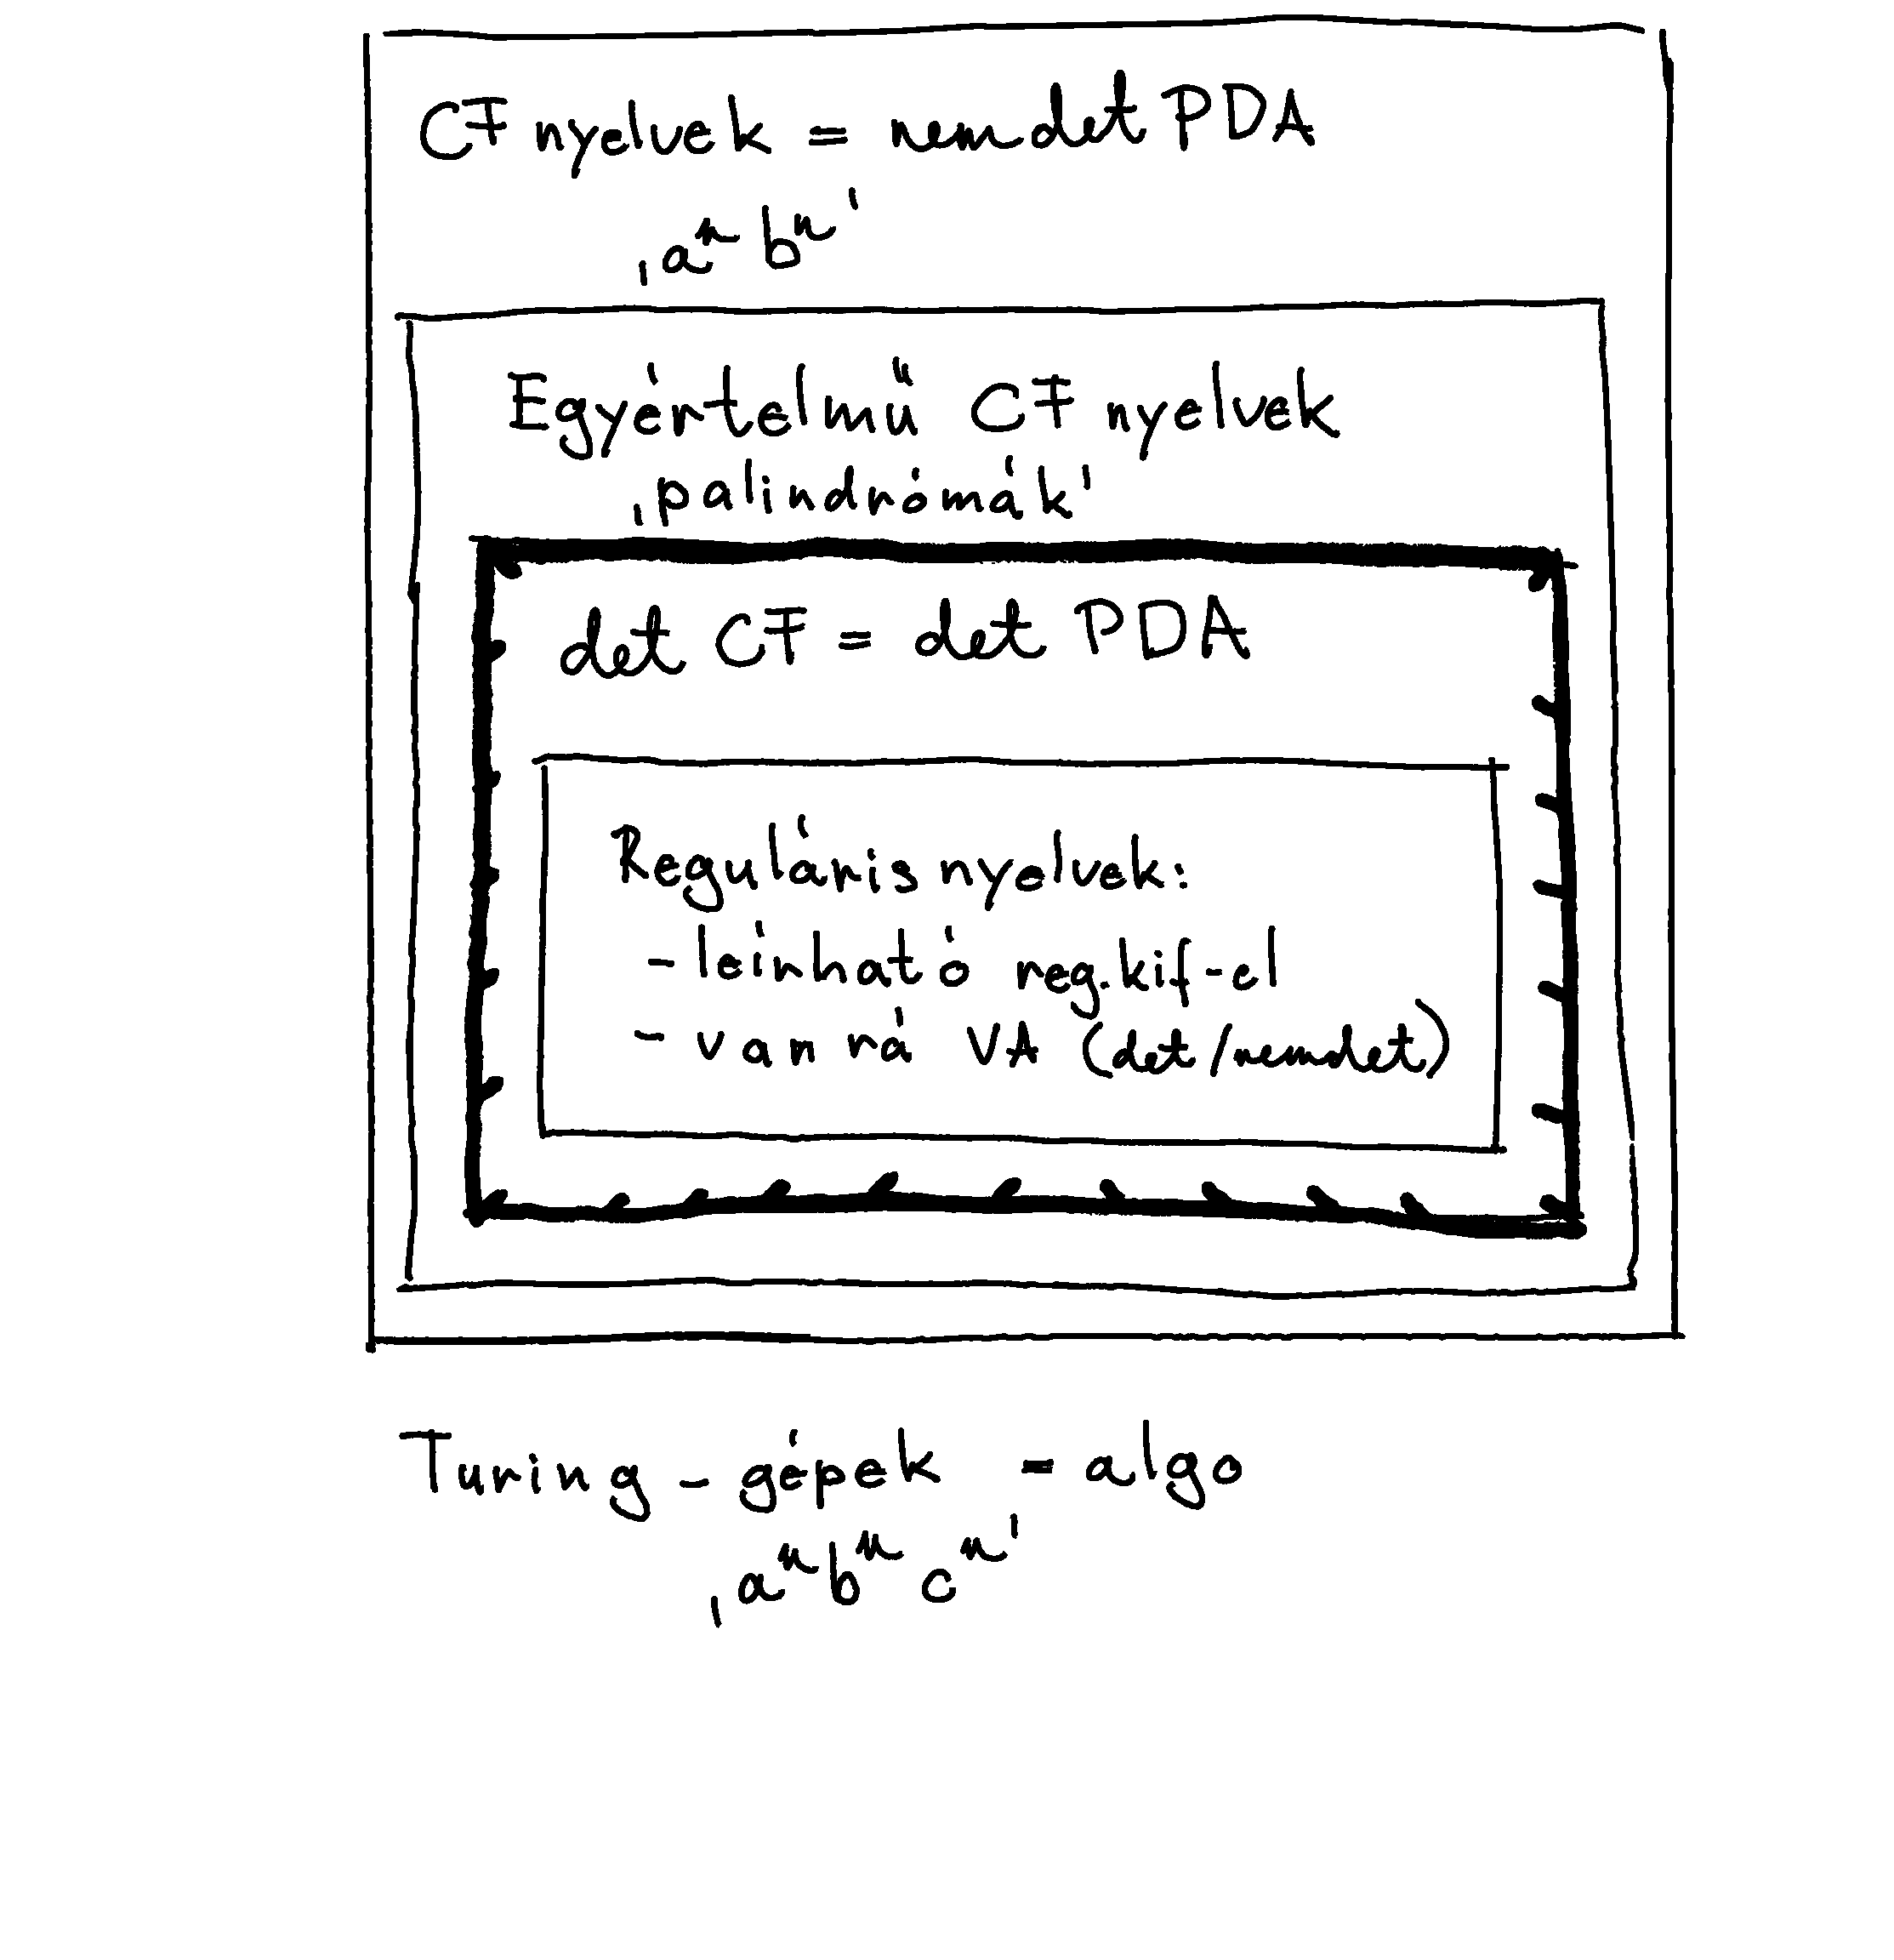
\includegraphics[scale=0.2]{images/image-1}
\end{center}

\begin{tcolorbox}[size = fbox]
  \textbf{Diagonális nyelv:} $L_d = \{ w \in \{0,1\}^*\ |\ \exists M_w $ ($w$ egy TG-et kódol) és $w \notin L(M_w)$ ($w$-t nem fogadja el a TG)$\}$ 
\end{tcolorbox}

\begin{tcolorbox}[size = fbox]
  \textbf{Állítás:} Nincs olyan $M$ TG amire $L(M) = L_d$
\end{tcolorbox}

\begin{tcolorbox}[size = fbox]
  \textbf{Megállási nyelv:} $L_h = \{ w\#s \ |\ w \in \{0,1\}^*, s \in \{0,1\}^*$ és $\exists M_w$ és $M_w$ leáll $s$-en$\}$ ($w\#s$ egy szópárt jelöl)
\end{tcolorbox}

\begin{tcolorbox}[size = fbox]
  \textbf{Állítás:} $L_h$-ra van TG de nincs \textbf{mindig leálló} TG.
\end{tcolorbox}

\begin{tcolorbox}[size = fbox]
  \textbf{Church-Turing tézis:} 
  \begin{enumerate}[label=(\roman*)]
    \item $L$ nyelvre van algoritmikus eljárás, ami éppen $L$ szavait fogadja el $\Longleftrightarrow$ $L$-re van $M$ TG: $L(M) = L$.
    \item $L$ nyelvre van mindig leálló algoritmus, ami $L$ szavait fogadja el $\Longleftrightarrow$ $L$-re van mindig leálló $M$ TG: $L(M) = L$.
  \end{enumerate}
\end{tcolorbox}

\begin{tcolorbox}[size = fbox]
  \textbf{Tétel:} $L$-re van $M$ nemdet TG: $L(M): L \Longleftrightarrow$ $L$-re van $M'$ det TG: $L(M'): L$.
\end{tcolorbox}

\begin{tcolorbox}[size = fbox]
  \textbf{P:} Azon $L$ nylevek, amelyekre van $M$ polinom időkorlátos det TG: $L(M) = L$
\end{tcolorbox}

\begin{tcolorbox}[size = fbox]
  \textbf{NP:} Azon $L$ nylevek, amelyekre van $M$ polinom időkorlátos nemdet TG: $L(M) = L$
\end{tcolorbox}

\begin{tcolorbox}[size = fbox]
  \textbf{coNP:} Azon $L$ nylevek, amelyeknek a komplementere NP-beli.
\end{tcolorbox}

\begin{tcolorbox}[size = fbox]
  \textbf{Tanú tétel:} $L \in $ NP akkor és csak akkor, ha $\exists c_1, c_2 > 0$ és $L_1$ szópárokból áll:
  \begin{enumerate}[label=(\roman*)]
    \item $L_1 \in $ P, azaz $(x, y)$ párról gyorsan eldönthető, hogy jó pár-e.
    \item $x \in L \Longleftrightarrow \exists y: |y| \leq c_1 \cdot |x|^{c_2}$ és $(x, y) \in L_1$. 
  \end{enumerate}
\end{tcolorbox}

\begin{tcolorbox}[size = fbox]
  \textbf{Tétel:} P $\subseteq$ coNP
\end{tcolorbox}

\begin{tcolorbox}[size = fbox]
  \textbf{Karp redukálhatóság:} $L_1$ és $L_2$ két $\{0,1\}^*$-beli nyelv. $L_1 \prec L_2$ : $L_1$ Karp-redukálható $L_2$-re, ha $\exists f: \{0,1\}^* \rightarrow \{0,1\}^*$ és
  \begin{enumerate}[label=(\roman*)]
    \item $f$ minden $\{0,1\}^*$-beli szón értelmezett
    \item $f(x)$ gyorsan számolható: O$(|x|^{c_1})$ időben
    \item $x \in L_1 \Longleftrightarrow f(x) \in L_2$.
  \end{enumerate}
\end{tcolorbox}

\begin{tcolorbox}[size = fbox]
  \textbf{NP teljes:} $Y$ probléma NP-teljes, ha:
  \begin{enumerate}[label=(\roman*)]
    \item $Y \in $ NP
    \item $\forall X \in$ NP : $X \prec Y$
  \end{enumerate}
\end{tcolorbox}

\end{document}